\chapter{Methodology} \label{chp:3}
%%%%%%%%%%%%%%%%%%%%%%%%%%%%%%%%%%%%%%%%%%%%%%%%%%%%%%%%%%%%%%%%%%%%%%%
With an entire field of data-mining established around methods of gathering knowledge from large data-sets. The development of a first generation database mining-system will serve as an outline towards an automated approach \cite{Imielinski1996, Radivojac2004, Uppalaiah2012}. These outlines are set forth in terms of four objectives.

\begin{enumerate}
\item Data processing
\item Transformation
\item Analysis
\item Visualization
\end{enumerate} 

These sections will therefore follow this outline, with reference to figure \ref{dataFlow}, in detailing the methods involved.

\begin{figure}[h] \label{dataFlow}
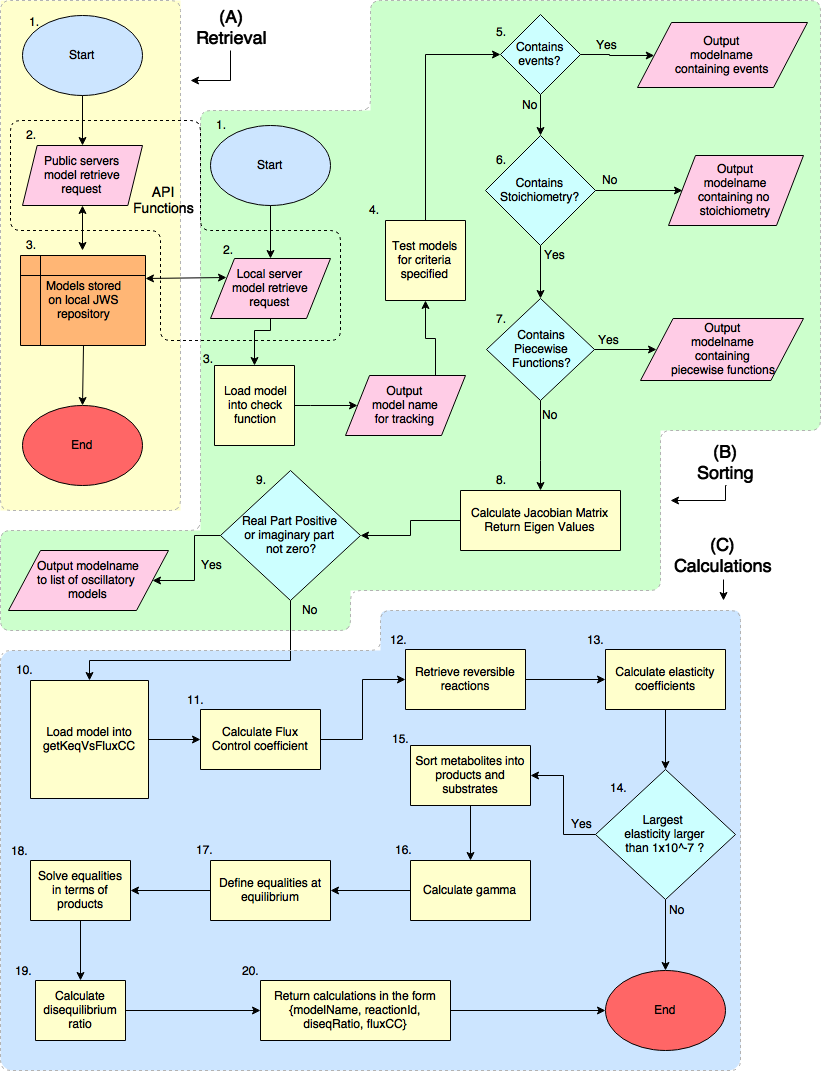
\includegraphics[width=1\textwidth]{Algorithm.png}
\centering
\caption{Overview diagram of algorithm indicating the flow of data throughout the run-time}
\label{fig:Algorithm}
\end{figure}

\section{Data processing} \label{Data processing}
Data processing refers to the act of information retrieval, conducted in a manner that is conducive to the transformation processes that will follow. With reference to figure \ref{dataFlow}, data processing entails the retrieval (A) and sorting (B) methods, as discussed in sections \ref{Retrieval} and \ref{Sorting}. For now however, the focus will be on the initial set up of the working environment used.

\section{Setting up the Working environment} \label{Working Environment}
The working environment was constructed in two parts, a data management component and a scripting language. The data management component is responsible for storing and translating model information, whilst the scripting language provides automation of compute operations required. These components were fulfilled by a local instance of \href{https://jjj.bio.vu.nl}{JWSOnline} and Mathematica v11 respectively. The JWSOnline server instance is hosted through the Docker platform, discussed in section \ref{Docker Installation}. For a more complete JWSOnline docker installation guide please refer to the documentation, available at \href{http://jws-docs.readthedocs.io/10_docker.html#building-the-jws-online-docker-image}.

\subsection{JWSOnline and Docker installation} \label{Docker Installation}
Docker, an open source platform, had the advantage of being platform agnostic. As such a Docker environment is self contained and easily reproducible, an advantage and requirement towards scientific inquiry. The main aim of a locally hosted \href{https://jjj.bio.vu.nl}{JWSOnline} server, was to achieve isolation from active production servers as to not inundate them with repetitive model upload, download, query and conversion operations. This proved especially useful considering the repetitive nature associated with a development and testing cycle for thousands of models. An added benefit was an observed increase in overall efficiency, taken as time to handle the entire data-set. This was due to internet connection speed and availability affecting only the initial retrieval of models from public servers. Overhead communication rates, between Mathematica and the server instance, was limited only by processor transfer rates. 

Starting out, the Docker host application is downloaded and installed for the operating system in question (OSX in this case) as instructed by the docker documentation available at \href{http://docker-sean.readthedocs.io}{http://docker-sean.readthedocs.io}. The JWSOnline Docker compose script, located at \href{http://jws-docs.readthedocs.io/10_docker.html#building-the-jws-online-docker-image} was copied and saved into a local file named "docker-compose.yml", noting the working directory. More information on the ".yml" format and the docker compose file in general can be obtained at \href{https://docs.docker.com/compose/compose-file/#compose-file-structure-and-examples} as a deeper description is outside of the scope of this thesis. 
Environment variables such as passwords and volume names in the "docker-compose.yml" is altered and saved to user specific requirements. This would be individual specific and other than the need for authentication the choice of these variables has no appreciable impact on further operations. Afterwards the images and services defined are retrieved by running the command "docker-compose pull" from within a terminal/bash environment (Please note this command must be performed from within the working directory noted earlier). The retrieved services are then launched by the "docker-compose up" command. This command starts the services as defined by the "docker-compose.yml" file. A successful installation and start up is confirmed by visiting the local host or loop back IP address (127.0.0.1) in a web browser and being greeted with a local JWSOnline homepage.

As mentioned earlier, the local JWSOnline installation provided the model handling portion of the working environment and as such needed to be able to communicate with the scripting language, Mathematica, at hand. The communications method native to JWSOnline, is in the form of a representational state transfer (REST) application program interface (API). As this is the basis of data transfer, the following section will provide a brief overview of example constructs, with specifics handled as applicable. 

\subsection{Communicating with JWSOnline via the \gls{rest} \gls{api}} \label{REST Communication}

The REST communications protocol allows applications and programs to share information with one another through a standardized method. A plethora of \gls{api} methods exist for various websites, but for the sake of simplicity the focus of this discussion will rest on the RESTFull web service framework \cite{rest2018}.

From a server perspective the \gls{rest} framework enables the control of access to internal application resources, while maintaining open access to services made available by such applications. These service endpoints are accessible to a client in the form of a basic URL request. This request uses the hypertext transfer protocol (HTTP) as is familiar from all generic web browsers. The REST framework was specifically developed in this way as to simplify the development process. Various applications can communicate with one another in a uniform manner \cite{rest2018}. Case and point, the availability of the \href{http://jjj.biochem.sun.ac.za}{JWSOnline} \gls{api} enabled the interaction of the web server with other applications or compute platforms, thus expanding the use of the application outside of the original project scope. 

HTTP requests can take on many forms, however for the purpose of this study the constructs will be fairly similar. For instance, one such example can take on the following form; \href{http://jjj.biochem.sun.ac.za/rest/models/teusink/mf}{http://jjj.biochem.sun.ac.za/rest/models/teusink/mf}. Various parts was interactively altered, as described in section \ref{Data processing}, in an attempt at an automated model handling algorithm. Let us therefore investigate and build upon this request. As is indicated by the "HTTP://" portion, this request utilizes the hypertext transport protocol (HTTP) at host address \href{jjj.biochem.sun.ac.za}{jjj.biochem.sun.ac.za}. The request is directed at the \gls{rest} endpoint within the "/models" directory to return the "/teusink" model in an "/mf" format. The returned result is a JSON data pair with model name and data contents as the first and second respective entries.

This example request above can be altered to return models based on specified criteria. For example, metabolic models can be returned by altering the request construct as follow; \href{http://jjj.biochem.sun.ac.za/rest/models/?id=&organism=&process=1&jwsmodel__model_type=}{\nolinkurl{http://jjj.biochem.sun.ac.za/rest/models/?id=\&organism=\&process=1\&jwsmodel\_\_model\_type=}}. In this request, "process=1" refers to models fulfilling the prerequisite of containing metabolic processes as defined by annotations from model creation and curation stages. A different one of these endpoints enabled the integration of models from an external source, to within the JWSOnline database. This proved useful in obtaining a larger sample size, as the \href{https://www.ebi.ac.uk/biomodels-main/}{BioModels} repository was consulted and integrated as described in section \ref{Data processing}. For more on JWSOnline specific REST endpoints, please refer to the JWSOnline documentation \cite{jwsdocs}. 


\subsection{Retrieval (A)} \label{Retrieval}
JWSOnline provides an endpoint for model retrieval from remote sources in the form of a restfull API. These The URL interaction functions of Mathematica, namely HTTPRequest and URLExecute, was used to construct a list of URLs linking to SBML models in both JWSOnline as well as Biomodels. The relevant parts of the example URL construct (\href{http://jjj.bio.vu.nl/rest/fetch/?type={type}&redirect={redirect}&remote={remote}}) was replaced by the remote URL's from the list created above. This command, initiated from the local JWSOnline instance, sequentially imported and converted each model to an internal data format. After which, these models were available for retrieval in any of the formats supported by JWSOnline. This raised the question of which model format would be best suited for the investigation at hand.

For the development of an automated algorithm, handling metabolic model analysis, a specific model format was needed. One that proved generic enough to facilitate the development of unattended automated functions, yet flexible enough to uniformly handle differences among models from various origins, destined for a diverse range of uses. As such five key aspects were identified as criteria for a suitable model format.

The model format had to: 
\begin{enumerate} \label{modelFormat}
  \item Consistently store similar data type at the same index - predictability
  \item Be easily understood by both humans and computers alike - ease of development
  \item Impart all of the information stored within the original model - consistency
  \item Keep information uniformly organized - accuracy
  \item Allow for direct computational interaction - accessibility
\end{enumerate}

\gls{sbml} provides a standardized structure to which biological models are kept. As such it seemed a logical first choice. However, although \gls{sbml} meets many of the requirements such as, predictability, accuracy and consistency, it does not meet all. This is due to the fact that \gls{sbml} makes complete sense to a computer, yet the syntax has a steep learning curve for the human eye. Combined with the fact that no native Mathematica \gls{sbml} parsing was supported at the time of development, the ease of development and accessibility aspects proved problematic. Therefore a method of model translation was called for. 

This translation process was achieved through the use of \href{https://jjj.bio.vu.nl}{JWSOnline}, whereby a \gls{sbml} model was retrieved from a remote server, converted and made available in matrix format (\gls{mf}) (One of the native JWSOnline data formats). In \gls{mf}, data is organized by content type. For example; rate-equations, metabolites, stoichiometry, parameter-sets and more are all grouped as nested lists, visually illustrated by figure \ref{fig:MatrixFormat}.  This format was chosen as it fulfilled all of the criteria as set out in list \ref{modelFormat}. It had the added advantage of enabling metabolic control calculations as discussed in section \ref{Calculations} to be done via matrix methods as described by \citeauthor{Hofmeyr2001}

Once a model has been handled by \href{https://jjj.bio.vu.nl}{JWSOnline},the end product of the translation process is made available as an \gls{api} endpoint allowing for the retrieval of the model. For example, the Teusink model can be found at \href{https://jjj.bio.vu.nl/rest/models/teusink/mf/}{https://jjj.bio.vu.nl/rest/models/teusink/mf/}. Additional resources to JWSOnline are available at \href{http://jws-docs.readthedocs.io/8_rest.html}{JWS Docs}. 

\begin{figure}[p]
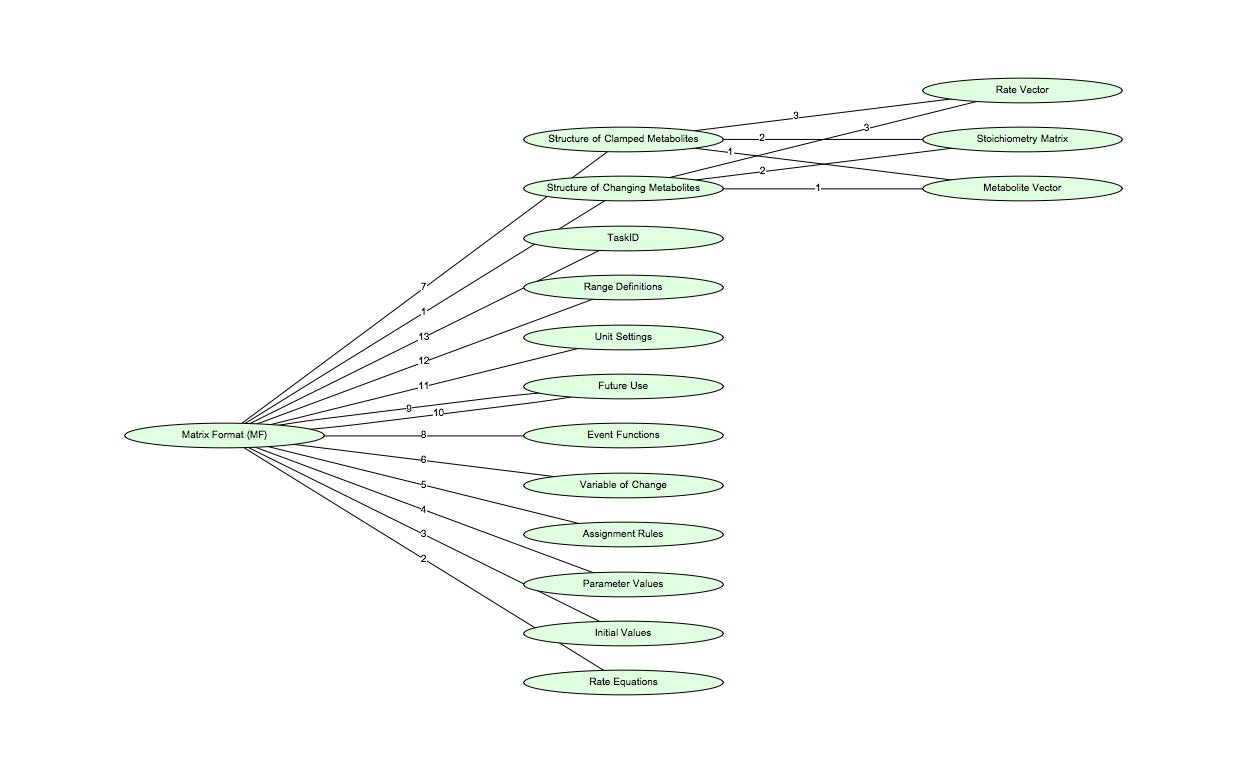
\includegraphics[width=1\textwidth]{MatrixFormat}
\centering
\caption{A graph representation of the Matrix Format (MF). Edge labels represent list index numbers and vertex labels denote content.}
\label{fig:MatrixFormat}
\end{figure}

\subsection{Sorting (B)}\label{Sorting}
Once all available models have been retrieved and stored within the local repository, the mf version was requested and returned as mentioned in section \ref{Retrieval}. These models then undergo a sorting and handling process, label B in figure \ref{fig:MatrixFormat}, in order to identify where models diverge from the main algorithm (3.). This process starts off by exporting the model name to a log file. Divergences in data flow was captured and visualized as discussed in chapter \ref{chp:4}. Vertices were defined as model and reaction names as well as endpoints specified. Edges in turn represented relationships and direction of procedural flow. Figure \ref{fig:MatrixFormat} was the end result of visualizing this log file and will be further discussed within section \ref{chp:4}. 

Once the initialization step was completed, a model was sent to a check function (4.). This function examines semantic structure as well as behaviour of models, in order to identify suitable models for the analysis at hand. The first process evaluates whether or not a model contains event functions. This is done by matching the pattern of an empty list to the appropriate sub list at index eight in the model (5.). A successful model is then checked for the presence of stoichiometry (6.). This is achieved by testing whether or not the stoichiometry list (index one) contains data. In other words, when the length of the list at the stoichiometry index is equal to zero, the model contains no stoichiometry and is handled and logged as such. Model event triggers, of the kind described above, can also be specified in terms of piece-wise functions (7.). As no a priori knowledge on the timing or the effect of these event triggers upon the steady state and control behaviour were available, they were also identified and logged. This identification was done based on the pattern of a reaction containing the string "Piecewise" as the function is referred to. 

These steps served as a minimal-validation for initial models. The order of operation proved important, as these procedures were not as computationally intensive as simulation and calculation operations. Therefore computational efficiency was gained in optimizing the order of operations. 

Following the semantic and structural tests described above, the stability of a model had to be assessed. This was done by evaluating model steady state behaviour. For this purpose the Jacobian matrix was consulted (8.). As is known from linear algebra, the eigenvalues of a Jacobian matrix holds information on the stability of a system of ODE's. The system is said to converge to a stable state when a decrease in perturbation is observed, in other words, from the jacobian matrix, real parts of eigenvalues are negative pointing to a decrease in initial perturbations. In contrast a positive eigenvalue points to a divergence from a stable state, as a perturbation is amplified. A third condition was the occurrence of a positive eigenvalue with a non zero imaginary part. These results are indicative of a system oscillating around some state, be it stable or unstable periodic behaviour. As such, model names exhibiting oscillatory behaviour were identified and written to our log file. For a simple test of stability, a Jacobian matrix that is invertible could serve as a positive test of steady-state \cite{Hofmeyr2001}.  

A model that have reached this point in the algorithm marked a checkpoint and was written, in full mf format, to a text file for record and future uses. Next up the model was sent for the simulation and calculation procedures as is described in the following section and as can be seen in figure \ref{dataFlow} number ten.


Biological model analysis platforms range from stand-alone applications, the likes of Jarnac, COPASI, CellDesigner and BioNetGen, to  add-on modules and libraries such as LibRoadRunner, COBRA, Pysces, SimBiology and Simulink, for the Python and Matlab scripting languages respectively \cite{Sauro2000, Hoops2006, Olivier2005, Somogyi2015, Harris2016, Laurent2017}. JWSOnline is a web based interactive interface for model creation, curation and simulation. A task achieved by utilizing custom Mathematica model manipulation packages alongside a combination of the above mentioned add-on modules, as described by \cite{Olivier2004, jwsdocs}. The JWSOnline platform is specifically mentioned here as it will form as a basis of tools, as described in section \ref{Working Environment} and \ref{Data processing}. 

The tools mentioned above, along with protocols and endpoints discussed in \ref{Working Environment}, prove useful in single isolated instances. However, when paired with scripting languages they can become immensely powerful and endlessly more useful. This is because automated computational operations can be performed faster, more accurately and for longer periods of time than would be otherwise possible by human minds. The following section is therefore dedicated to the introduction and explanation of individual steps, leading up to the entirety of such an automated model interrogation algorithm responsible for the collection of data utilized in the analysis, described in section \ref{Analysis}. 










\subsection{Calculations (C)} \label{Calculations}
The \gls{steady-state} of a model was calculated and the flux control coefficients were determined (10.). This was done utilizing linear algebra methods as described by \citeauthor{Hofmeyr2001}. This method entails the reduction of a stoichiometry matrix $N$ to row echelon form by Gaussian elimination. The reduced matrix $N_R$ contains the independent reactions and can be returned to $N$ matrix by defining a link matrix $L$ such that $N = LN_R$. Further information on the dependent and independent relationships are possible, yet will not be discussed here. 

Elasticity co\"efficients $\Bar{\mathcal{E}}$ were determined by taking the partial derivatives of reaction rates with respect to steady state concentrations. This notation stems from the article by \citeauthor{Hofmeyr2001} with the bar on $\mathcal{E}$ indicating unscaled elasticities. Scaling can be applied in order to generate dimensionless elasticities $\mathcal{E}$. As mentioned earlier, the steady state is influenced by parameters populated from experimental procedures and as such, each steady-state is unique to parameter values and initial conditions. 

A steady-state consists of metabolite concentrations $s$ as well as flux through values $J$. Changes to these steady-state values $(s,J)$, due to perturbations of parameter $p$, can be approximated by the following means. For metabolite concentrations $s_2 = s_1 + \frac{\partial s}{\partial p}(p_2 - p_1)$ and fluxes $J_2 = J_1 + \frac{\partial J}{\partial p}(p_2 - p_1)$. 

From the above matrices, the flux control co\"efficients were determined. The product of $N_R\Bar{\mathcal{E}}L$ being defined as the Jacobian matrix $M$. Further discussions on the Jacobian matrix will follow. For now however the importance lies in the calculation of concentration control co\"efficients towards the end of determining flux control co\"efficients.

The concentration control co\"efficients indicate a measurement of, as the name suggests, relative changes to metabolite concentrations $s$ brought about by parameter perturbations $p$. From the matrix formalism the concentration control co\"efficients $\Bar{C^s}$ can be determined from the link matrix $L$ the Jacobian matrix $M$ and the reduced stoichometry matrix $N_R$ as $\Bar{C^s}=-LM^{-1}N_R$. Flux control co\"efficients were then calculated via the following equation $\Bar{C}^J = \Bar{\mathcal{E}_s}\Bar{C^s}+ I_n$ \cite{Hofmeyr2001}.

From the above, many results were generated and as such filtering and sorting proceeded with models containing negative flux control coefficients upon themselves. A perturbation, towards flux control co\"efficient determination, is considered as an increase or decrease in enzyme activity or concentration. Therefore a negative flux control was deemed improbable, as an increase in enzyme concentration would logically not lead to a decrease in reaction rate. No further investigation into this was committed as this is outside the scope of this thesis.

Considering that disequilibrium ratio calculations are only applicable within reactions proceeding in a reversible manner, a test function was developed to identified these reactions. A reversible reaction was defined as a rate equation containing a negative part within the numerator portion. This was drawn from general reaction rates where $v_{net} = v_{forward} - v_{reverse}$ thus allowing a rate to become negative (reversible) under appropriate conditions. The numerator is therefore recast into base components and tested for the presence of a negative-one term (12.). This was achieved by utilizing the tree form structures available to Mathematica leading to an equation expanded to smallest component parts. The position of these reversible reactions were then stored in a variable for use in disequilibrium calculations later. 

As can be seen from the calculations of flux control co\"efficients prior, an inverse of the Jacobian matrix is calculated (13.) \citeauthor{Hofmeyr2001}. Therefore, as the Jacobian approaches zero, an inverse would approach infinity. This introduced errors due to machine precision digit and accuracy limitations when elasticity values were too small. As such a further step in ensuring model validity was implemented via elasticity calculation checks. Maximum elasticity values of the system were compared to a threshold, chosen as $1 \cdot 10^{-10}$. The choice of this threshold was based on observation of failed calculations from models in a "trial and error manner".  Models surpassing this threshold was passed to the following step (14.). 

To calculate disequilibrium ratios, knowledge of metabolite identity (substrate/product) was needed. Metabolites were identified through the use of the stoichiometry matrix. One can extract products and substrates on the basis of stoichiometry values that are larger or smaller than zero respectively(15.). Returning a reaction id linked to product id allowed for the consistent handling of applicable reactions. In the case of multiple products only the first product was returned for use, more were not required. Once products have been identified, gamma was determined by raising each metabolite in a reaction to the power of it's corresponding stoichiometry, leading to the first part of symbolic gamma construction. From vector 
\[
S
=
\begin{bmatrix}
    s_{1} \\
    s_{2} \\
    s_{3} \\
    \vdots \\
    s_{n} 
\end{bmatrix}
\]

each component is raised to the corresponding collumn value from

\[
N 
=
\begin{bmatrix}
    x_{11} & x_{12} & x_{13} & \dots  & x_{1n} \\
    x_{21} & x_{22} & x_{23} & \dots  & x_{2n} \\
    \vdots & \vdots & \vdots & \ddots & \vdots \\
    x_{d1} & x_{d2} & x_{d3} & \dots  & x_{dn}
\end{bmatrix}
\]

leading to 

\[
S^N
=
\begin{bmatrix}
    s_1^{x_{11}} & s_2^{x_{12}} & s_3^{x_{13}} & \dots  & s_n^{x_{1n}} \\
    s_1^{x_{21}} & s_2^{x_{22}} & s_3^{x_{23}} & \dots  & s_n^{x_{2n}} \\
    \vdots & \vdots & \vdots & \ddots & \vdots \\
    s_1^{x_{d1}} & s_2^{x_{d2}} & s_3^{x_{d3}} & \dots  & s_n^{x_{dn}}
\end{bmatrix}
\]


For the second part, each of these exponents were multiplied by one another according to the respective reaction rows 

\[
V
=
\begin{bmatrix}
    V_{1} \\
    V_{2} \\
    \vdots \\
    V_{d} 
\end{bmatrix}
\]

such that

\[
\gamma 
=
\begin{bmatrix}
    s_1^{x_{11}}s_2^{x_{12}}s_3^{x_{13}} \dots s_n^{x_{1n}} \\
    s_1^{x_{21}}s_2^{x_{22}}s_3^{x_{23}} \dots s_n^{x_{2n}} \\
    \vdots\\
    s_1^{x_{d1}}s_2^{x_{d2}}s_3^{x_{d3}}\dots s_n^{x_{dn}}
\end{bmatrix}
\]

From the above it can be seen that stoichiometries of zero will result in power calculations of one. With negative and positive stoichiometries as denominators and numerators respectively, resulting in the gamma fraction \gamma of the specific reaction. $K_{eq}$ calculations where done, as an example from the Tuesink model mention earlier. The 2-Phospho-D-glycerate 2,3-phosphomutase catalyzed reaction leading from P2G to PEP is used as an example, where an equality is defined in terms of equilibrium, \textit{i.e.} the rate equation $v_n$ equals zero.

\begin{equation}
v = \frac{V_mENO([P2G] - \frac{[PEP]}{K_{eq}ENO})}{K_mENOP2G(1 + \frac{[P2G]}{K_mENOP2G} + \frac{[PEP]}{K_mENOPEP})} = 0
\end{equation}

Following this, the equality was symbolically solved in terms of the product identified in (15.). In the example case PEP is the product. As such the above equation in terms of PEP becomes

\begin{equation}\label{PEP}
PEP = K_{eq}ENOP2G
\end{equation}

From the calculations above, this reaction has

\begin{equation}\label{gamma}
\gamma=\frac{[PEP]^1}{[P2G]^1}
\end{equation}

Substitution of equation \ref{PEP} into \ref{gamma} yields $\gamma$ at equilibrium, otherwise known as $K_{eq}$. Therefore

\begin{equation}\label{Keq}
K_{eq}=K_{eq}ENO
\end{equation}

Taking equation \ref{gamma} divided by \ref{Keq} gives us the disequilibrium ratio
\begin{equation}
\rho = \frac{\gamma}{K_{eq}} = \frac{\frac{[PEP]^1}{[P2G]^1}}{K_{eq}ENO}
\end{equation}

Substituting steady-state values allows for the calculation of the numerical disequilibrium ratio. This was the generic manner in which disequilibrium calculations were done. From this methods described, two values were returned per reaction. The flux control co\"efficient as well as the disequilibrium ratio. These results were used further towards the analysis at hand.

\section{Analysis} \label{Analysis}
